% Provenance (never printed): see sources/outline_sources.md (Year 1: continental
% rifting and break-up; passive-margin structure; fast and slow ridges; the depth--age
% law of the ocean floor; transform faults). Curve from figdata/bachelor-1/depth_age.py;
% exercise and problem values in the Book 3 scratch calculator calc/ch13.py; the
% coordinates of the margin schematic from calc/fig13_margin.py.
\chapter{الشقوق والحيود والهوامش السلبية}\label{ch:b1:rifts-ridges-margins}

في سبتمبر 2005 انفتحت أرض صحراء عفار، في شمال شرق إثيوبيا. وخلال ثلاثة أسابيع اتّسع جزء من الشقّ، طوله نحو \qty{60}{km}، بما يصل إلى \qty{8}{m}، وصعد نحو \qty{2.5}{km^3} من الصهارة إلى الصدع من أسفل. وتنفصل الصفائح هناك بنحو \qty{18}{mm} في السنة: فالأزمة أطلقت، في بضعة أسابيع، تمدّد نحو أربعة قرون. عفار قارة تتمزّق؛ وعلى بضع مئات من الكيلومترات شمالًا، البحر الأحمر محيط فتيّ يُصنع قاعه بالفعل كقاع الأطلسي، وكان الأطلسي الجنوبي شقًّا من هذا القبيل قبل أن ينفتح، قبل نحو 120 مليون سنة. يتتبّع هذا الفصل ولادة محيط: تمدّد قارة، وانشقاقها، والهامشين السلبيين اللذين يتركهما، والحيد الذي يبني قاع المحيط، والهبوط البطيء لذلك القاع مع تبرّده.
% ledger: wright:afar, morvel:ar-nb (18.5 mm/yr at 12.3 N, 40.6 E, computed with euler_velocities.py), heine:fit

\begin{recall}
الصفائح هي \omterm{def:b1:heat-budget:boundary-layer}{الطبقة الحدّية الحرارية} العليا \omterm{def:b1:layered-earth:layers}{للوشاح}؛ وتحت المحيطات يصفها نصف فضاء يبرد، وتتعمّق متساوياتها الحرارية كجذر العمر (\cref{ch:b1:heat-budget}). وأعمدة الصخر في توازن أيزوستاتي لها الكتلة نفسها لكل وحدة مساحة فوق \omterm{def:b1:isostasy-gravity:isostasy}{عمق التعويض} (\cref{ch:b1:isostasy-gravity}). وتدور الصفائح حول أقطاب أويلر، وتنتشر الحيود بمعدّلات تُقرأ من الشذوذات المغناطيسية، والصدوع التحويلية تقع على دوائر صغرى حول القطب (\cref{ch:b1:plate-kinematics}). وقد عُرّفت \omterm{def:b1:cross-sections:throw}{الإزاحة الرأسية} \omterm{def:b1:cross-sections:throw}{والإزاحة الأفقية} لصدع في \cref{ch:b1:cross-sections}؛ والصدع العادي صدع مائل تحرّكت كتلته العليا إلى الأسفل (الكتاب 2، الصف 11).
\end{recall}

\section{الانشقاق القاري}

القارة التي تتمدّد بقوى على حوافها لا تترقّق بانتظام. \omterm{def:b1:layered-earth:layers}{فالقشرة} العليا الهشّة تنكسر على طول صدوع عادية، وتهبط الكتل المحصورة بينها وتميل؛ وتحتها تتدفّق \omterm{def:b1:layered-earth:layers}{القشرة} السفلى الأدفأ \omterm{def:b1:layered-earth:layers}{والوشاح}.

\begin{definition}[الشقّ القاري، الغرابن، نصف الغرابن]\label{def:b1:rifts-ridges-margins:rift}
\emph{الشقّ القاري}\index{الشقّ القاري} منطقة طويلة ضيقة تتمدّد فيها قارة: منخفض تحدّه صدوع عادية، مع زلازل وكثير من البراكين في الغالب. و\emph{الغرابن}\index{الغرابن} كتلة هابطة بين صدعين عاديين يميلان أحدهما نحو الآخر. و\emph{نصف الغرابن}\index{نصف الغرابن} كتلة هابطة ومائلة نحو صدع عادٍ رئيس واحد، هو صدع الحدّ، على جانب واحد فقط.
\end{definition}

تتألف معظم أحواض الشقوق من سلاسل من أنصاف \omterm{def:b1:rifts-ridges-margins:rift}{الغرابن}. وتنقل صدوع حدودها الإزاحة من واحد إلى الآخر عبر منحدرات الترحيل، وكثيرًا ما يتناوب جانب صدع الحدّ من قطعة إلى التي تليها. ويميل الجدار المعلّق لكل صدع حدّ نحوه، ويمتلئ الحوض أسرع ما يكون هناك: فأسمك الرواسب يتراكم عند الصدع، بينما يُرفع الجدار الراقد إلى كتف الشقّ.

التمدّد الأفقي الذي يحمله الصدع هو \omterm{def:b1:cross-sections:throw}{إزاحته الأفقية}. وصدع عادٍ مستوٍ إزاحته الرأسية $h$ وانحداره $\delta$ \omterm{def:b1:cross-sections:throw}{إزاحته الأفقية} $h/\tan\delta$ (\cref{ch:b1:cross-sections})؛ وجمع الإزاحات الأفقية للصدوع عبر مقطع شقّ يعطي امتداد \omterm{def:b1:layered-earth:layers}{القشرة} الهشّة. أما كيف ينحسف \omterm{def:b1:layered-earth:lithosphere}{الغلاف الصخري} كله مع تمدّده، ولماذا يهبط بعد ذلك، فيُقاس في الكتاب 4؛ وهنا تُقاس الصدوع، ويُقارن مجموعها بحركة الصفائح.

\begin{omfigure}
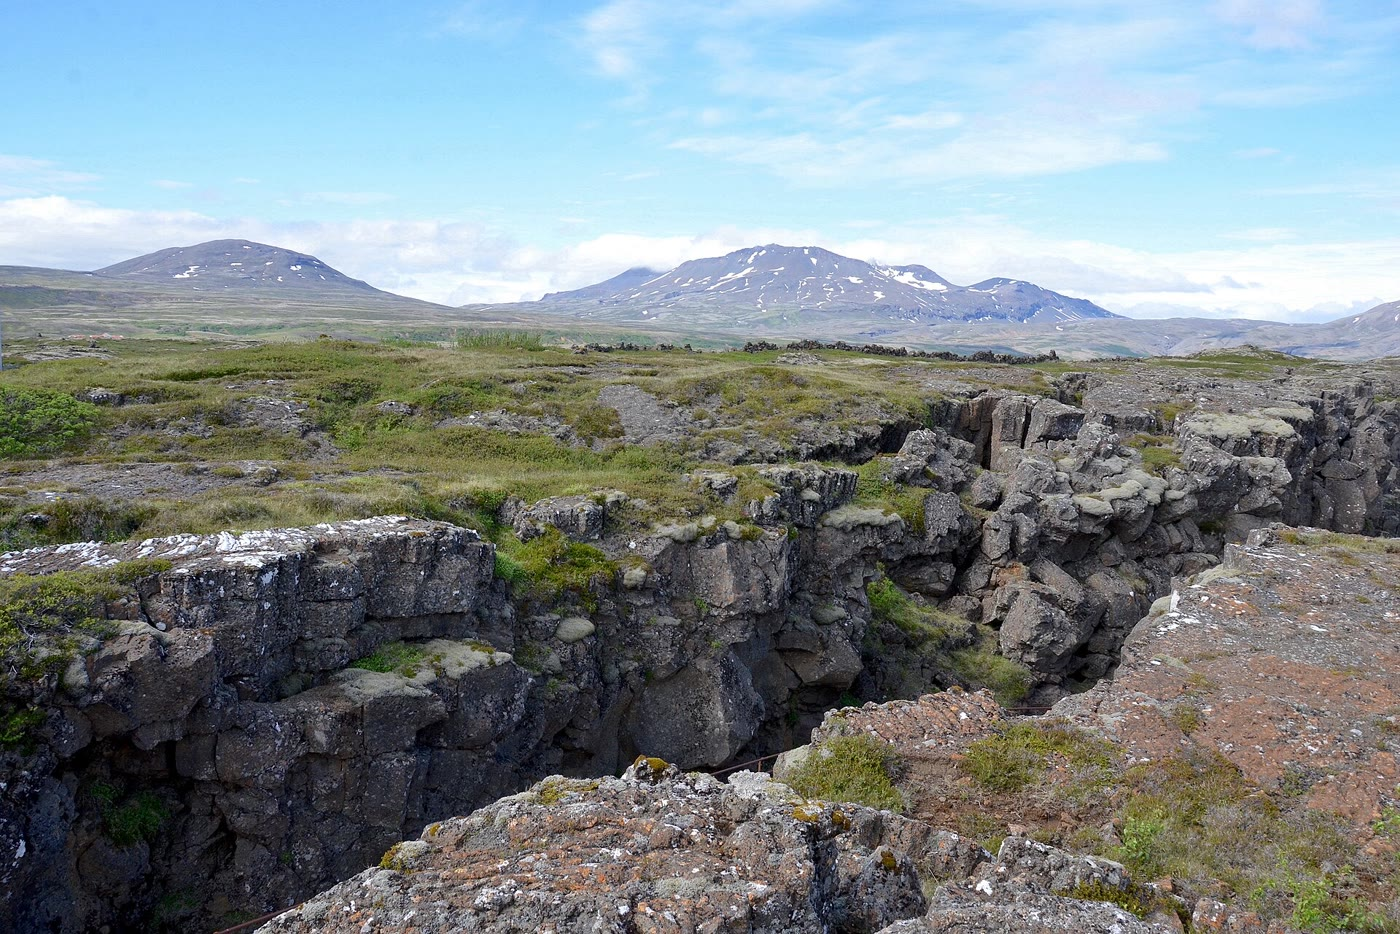
\includegraphics[width=0.8\linewidth]{images/book3/b1-thingvellir-fissure.jpg}

\par\smallskip{\small شقّ مفتوح في أرضية الحمم بوادي شقّ ثينغفيلير، في جنوب غرب أيسلندا، حيث يصل الحيد الأطلسي الأوسط إلى اليابسة. وتقطع تدفّقات البازلت في قاع الوادي شقوقٌ مفتوحة موازية للشقّ. الصورة: Olga Ernst، CC~BY-SA~4.0 (Wikimedia Commons).}
\label{fig:b1:rifts-ridges-margins:thingvellir}
\end{omfigure}
% ledger: commons:thingvellir

\subsection*{الشقوق البركانية والشقوق الفقيرة بالصهارة}

تختلف الشقوق في مقدار الصهارة التي تتلقاها. ففي شقّ \emph{فقير بالصهارة} يتحمّل الصدوع التمدّد، وتترقّق \omterm{def:b1:layered-earth:layers}{القشرة} مع انزلاق الكتل بعيدًا عن بعضها. وفي شقّ بركاني تتولّى الصهارة الأمر: إذ تتسلّل السدود إلى \omterm{def:b1:layered-earth:layers}{القشرة} على امتداد المحور، كلٌّ منها يفتح الشقّ بسمكه، وتغمر الحمم السطح. ويجمع شقّ أفريقيا الشرقي الاثنين جنبًا إلى جنب: ففرعه الشرقي بركاني بقوة، بينما فرعه الغربي أقلّ بركانية ويحوي أحواضًا رسوبية عميقة، تملؤها بحيرات مثل بحيرة تنجانيقا، ويحدّها صدوع.
% ledger: roberts:ear

بدأ الفرعان في التكوّن قبل نحو 25 مليون سنة، ويقسم الشقّ الصفيحة الأفريقية إلى صفيحة نوبية غربًا وصفيحة صومالية شرقًا. ومن مفصل عفار الثلاثي يمتد جنوبًا، في فرعين يلتفّان حول كراتون تنزانيا القديم السميك البارد. وحركته بطيئة: فمحسوبةً من متجهتي الصفيحتين الصومالية والنوبية، كل منهما مقاسة بالنسبة إلى الصفيحة القطبية الجنوبية، تبتعد الصومالية عن النوبية بمعدّل \qty{6.0}{mm.yr^{-1}} نحو \ang{105} في وسط إثيوبيا (\ang{8.5}~ش، \ang{39.5}~ق)، وبمعدّل \qty{5.1}{mm.yr^{-1}} عند خط الاستواء. وتُظهر زلازل كثيرة للشقّ انكسارًا عاديًا.
% ledger: roberts:ear, morvel:sm-an, morvel:nb-an (SM-NB from SM-AN minus NB-AN, computed with figdata/bachelor-1/euler_velocities.py)

وفي عفار، عند طرفه الشمالي، يلتقي الشقّ بالبحر الأحمر وخليج عدن. فمعظم البازلت الفيضي الإثيوبي اندفع هناك قبل نحو 30 مليون سنة، في مليون سنة أو أقل، ولم تتوقف الصهارة عن الوصول منذ ذلك الحين: حمم تتدفّق على السطح، وتسلّلات في \omterm{def:b1:layered-earth:layers}{القشرة}، ومادة جديدة تُضاف تحتها، حتى إن \omterm{def:b1:layered-earth:layers}{القشرة} المخترقة حافظت على سمكها خلال المراحل الأولى من الانشقاق. وتُظهر أزمة 2005 كيف ينفتح شقّ كهذا: لا بثبات، بل بنوبات، كلٌّ منها سدّ عرضه أمتار يتسلّل خلال أيام أو أسابيع. ولأن الصفائح تتباعد هناك بنحو \qty{18}{mm.yr^{-1}}، فإن السدّ البالغ \qty{8}{m} سنة 2005 استوعب تمدّد نحو 440 سنة.
% ledger: hofmann:traps, bastow:afar, wright:afar, morvel:ar-nb (rate computed with euler_velocities.py)

\section{الانفصال والهوامش السلبية}

إذا تواصل التمدّد، تترقّق \omterm{def:b1:layered-earth:layers}{القشرة} القارية حتى تنعدم، ويرتفع \omterm{def:b1:layered-earth:layers}{الوشاح} تحت الشقّ فيذوب وهو يصعد، وتتكوّن أول \omterm{def:b1:rifts-ridges-margins:oceanic-crust}{القشرة المحيطية} بين شطرَي القارة. وتلك اللحظة هي \emph{الانفصال}. ومن ذلك الحين تتباعد الصفائح عند حيد في وسط محيط جديد، وتكفّ حافتا القارة، المحمولتان بعيدًا عن الحيد، عن أن تكونا حدّي صفيحتين.

\begin{definition}[الهامش السلبي؛ الانتقال من المحيط إلى القارة؛ عدم التوافق عند الانفصال]\label{def:b1:rifts-ridges-margins:passive-margin}
\emph{الهامش السلبي}\index{الهامش السلبي} هو حافة قارة تشكّلت بالانشقاق ولم تعد حدّ صفيحة: فالقارة وقاع المحيط المجاور ينتميان إلى الصفيحة نفسها. و\emph{الانتقال من المحيط إلى القارة}\index{الانتقال من المحيط إلى القارة} هو منطقة الهامش، عرضها من كيلومترات إلى عشرات الكيلومترات، بين \omterm{def:b1:layered-earth:layers}{قشرة} قارية مترقّقة \omterm{def:b1:layered-earth:layers}{وقشرة} محيطية عادية. و\emph{عدم التوافق عند الانفصال}\index{عدم التوافق عند الانفصال} هو \omterm{def:b1:cross-sections:unconformity}{عدم التوافق} الذي يفصل الرواسب التي تراكمت في أحواض الشقّ، مائلةً مع كتلها، عن الرواسب غير المضطربة التي استقرّت فوق الهامش بعد الانفصال.
\end{definition}

تصطفّ الهوامش السلبية على معظم الأطلسي والمحيط المتجمد الشمالي والمحيط الهندي الغربي، وعلى معظم سواحل أفريقيا وأستراليا وغرينلاند والهند. والحافة الشرقية لأمريكا الشمالية والحافة الشمالية الغربية لأفريقيا كانتا جانبي شقّ واحد: إنهما هامشان \emph{متقابلان}. وقطاعهما هو التتابع المألوف لقاع المحيط قرب اليابسة: الرفّ القاري، فالمنحدر، فالمرتفع، فالسهل القاعي. وتحت الرفّ والمنحدر يرقد الغلاف القاري المترقّق، تقطعه صدوع عادية تميل نحو المحيط، وكتله المدارة مدفونة تحت الرواسب.

\begin{omfigure}
\begin{tikzpicture}[x=0.95cm, y=0.9cm, font=\scriptsize]
% (a) continental rift: half-grabens on east-dipping faults; coordinates from calc/fig13_margin.py
\begin{scope}
\fill[green!25!gray!45] (0,-2) -- (3,-2) -- (6,-1.75) -- (9,-2) -- (12,-2) -- (12,-2.5) -- (0,-2.5) -- cycle;
\fill[orange!22] (0,0) -- (3.5,0) -- (3.931,-0.8) -- (4.75,-0.25) -- (5.05,-0.7) -- (6,-0.2) -- (6.223,-0.55) -- (7.25,-0.15) -- (7.402,-0.4) -- (8.6,0) -- (12,0) -- (12,-2) -- (9,-2) -- (6,-1.75) -- (3,-2) -- (0,-2) -- cycle;
\fill[yellow!45] (3.565,-0.12) -- (3.931,-0.8) -- (4.75,-0.25) -- (4.75,-0.12) -- cycle;
\fill[yellow!45] (4.75,-0.12) -- (4.75,-0.25) -- (5.05,-0.7) -- (6,-0.2) -- (6,-0.12) -- cycle;
\fill[yellow!45] (6,-0.12) -- (6,-0.2) -- (6.223,-0.55) -- (7.25,-0.15) -- (7.25,-0.12) -- cycle;
\fill[yellow!45] (7.25,-0.12) -- (7.25,-0.15) -- (7.402,-0.4) -- (8.241,-0.12) -- cycle;
\draw (0,0) -- (3.5,0) -- (3.931,-0.8) -- (4.75,-0.25) -- (5.05,-0.7) -- (6,-0.2) -- (6.223,-0.55) -- (7.25,-0.15) -- (7.402,-0.4) -- (8.6,0) -- (12,0);
\draw[contact] (0,-2) -- (3,-2) -- (6,-1.75) -- (9,-2) -- (12,-2);
\draw[fault] (3.5,0) -- (4.2,-1.3);
\draw[fault] (4.75,-0.25) -- (5.45,-1.3);
\draw[fault] (6,-0.2) -- (6.7,-1.3);
\draw[fault] (7.25,-0.15) -- (7.95,-1.3);
\node[anchor=west, font=\small\bfseries] at (0,0.75) {(أ) الشقّ القاري};
\node[anchor=south] at (2.2,0) {كتف الشقّ};
\node[anchor=south, align=center] at (6.3,0) {أنصاف الغرابن المملوءة بالرواسب};
\draw[-{Stealth[length=3pt]}] (2.6,-0.75) node[anchor=east] {صدع الحدّ} -- (3.75,-0.5);
\node at (9.8,-1.0) {القشرة القارية};
\node at (10.3,-2.25) {الوشاح};
\node at (6,-2.18) {موهو مرتفع تحت الشقّ};
\end{scope}
% (b) break-up: conjugate halves, the first oceanic crust between them
\begin{scope}[yshift=-3.6cm]
\fill[omSea!35] (2.8,0) -- (9.2,0) -- (9.2,-1.3) -- (2.8,-1.3) -- cycle;
\fill[green!25!gray!45] (0,-2) -- (2.5,-2) -- (5.5,-1.3) -- (6.5,-1.3) -- (9.5,-2) -- (12,-2) -- (12,-2.5) -- (0,-2.5) -- cycle;
\fill[orange!22] (0,0) -- (2.8,0) -- (3.146,-0.75) -- (3.8,-0.3) -- (4.13,-0.85) -- (4.7,-0.45) -- (5.053,-0.95) -- (5.5,-1) -- (5.5,-1.3) -- (2.5,-2) -- (0,-2) -- cycle;
\fill[orange!22] (12,0) -- (9.2,0) -- (8.854,-0.75) -- (8.2,-0.3) -- (7.87,-0.85) -- (7.3,-0.45) -- (6.947,-0.95) -- (6.5,-1) -- (6.5,-1.3) -- (9.5,-2) -- (12,-2) -- cycle;
\fill[lith basalt] (5.5,-1) -- (6.5,-1) -- (6.5,-1.3) -- (5.5,-1.3) -- cycle;
\draw (0,0) -- (2.8,0) -- (3.146,-0.75) -- (3.8,-0.3) -- (4.13,-0.85) -- (4.7,-0.45) -- (5.053,-0.95) -- (5.5,-1) -- (6.5,-1) -- (6.947,-0.95) -- (7.3,-0.45) -- (7.87,-0.85) -- (8.2,-0.3) -- (8.854,-0.75) -- (9.2,0) -- (12,0);
\draw[contact] (0,-2) -- (2.5,-2) -- (5.5,-1.3) -- (6.5,-1.3) -- (9.5,-2) -- (12,-2);
\draw[omSea!70!black] (2.8,0) -- (9.2,0);
\draw[fault] (2.8,0) -- (3.4,-1.3);
\draw[fault] (3.8,-0.3) -- (4.4,-1.3);
\draw[fault] (4.7,-0.45) -- (5.3,-1.3);
\draw[fault] (9.2,0) -- (8.6,-1.3);
\draw[fault] (8.2,-0.3) -- (7.6,-1.3);
\draw[fault] (7.3,-0.45) -- (6.7,-1.3);
\draw[omRidge, very thick, -{Stealth[length=3pt]}] (6,-2.3) -- (6,-1.45);
\node[anchor=west, font=\small\bfseries] at (0,0.75) {(ب) الانفصال};
\node[anchor=south] at (6,0) {البحر يغمر الشقّ};
\node[anchor=west] at (6.15,-2.1) {الوشاح يرتفع ويذوب};
\node[anchor=south, fill=white, fill opacity=0.8, text opacity=1, inner sep=1pt, align=center] at (6,-0.85) {أول قشرة\\محيطية};
\node at (1.4,-1.0) {كتل مائلة};
\node at (10.6,-1.0) {كتل مائلة};
\node at (1.4,-2.25) {الوشاح};
\end{scope}
% (c) one passive margin after drift
\begin{scope}[yshift=-7.4cm]
\fill[omSea!35] (1.2,0.3) -- (12,0.3) -- (12,-1.2) -- (8.2,-1.15) -- (6.4,-0.9) -- (4.6,0.1) -- cycle;
\fill[green!25!gray!45] (0,-2.3) -- (2,-2.3) -- (5.9,-1.8) -- (6.7,-2.1) -- (12,-2.1) -- (12,-2.7) -- (0,-2.7) -- cycle;
\fill[orange!22] (0,0.3) -- (1.2,0.3) -- (2.2,0) -- (3,-0.25) -- (3.259,-0.95) -- (4,-0.55) -- (4.286,-1.15) -- (4.9,-0.85) -- (5.233,-1.35) -- (5.9,-1.55) -- (5.9,-1.8) -- (2,-2.3) -- (0,-2.3) -- cycle;
\fill[pattern=crosshatch dots, pattern color=green!40!black] (5.9,-1.55) -- (6.4,-1.75) -- (6.7,-2.1) -- (5.9,-1.8) -- cycle;
\fill[lith basalt] (6.4,-1.75) -- (12,-1.75) -- (12,-2.1) -- (6.7,-2.1) -- cycle;
\fill[yellow!45] (3,-0.25) -- (3.259,-0.95) -- (4,-0.55) -- cycle;
\fill[yellow!45] (4,-0.55) -- (4.286,-1.15) -- (4.9,-0.85) -- cycle;
\fill[yellow!45] (4.9,-0.85) -- (5.233,-1.35) -- (5.9,-1.55) -- (5.9,-1.45) -- cycle;
\fill[yellow!15] (1.2,0.3) -- (4.6,0.1) -- (6.4,-0.9) -- (8.2,-1.15) -- (12,-1.2) -- (12,-1.75) -- (6.4,-1.75) -- (5.9,-1.55) -- (5.9,-1.45) -- (4.9,-0.85) -- (4,-0.55) -- (3,-0.25) -- (2.2,0) -- cycle;
\draw[black!45] (2.4,0.12) -- (4.8,-0.1) -- (6.6,-1.05) -- (8.4,-1.27) -- (12,-1.31);
\draw (1.2,0.3) -- (4.6,0.1) -- (6.4,-0.9) -- (8.2,-1.15) -- (12,-1.2);
\draw[omSea!70!black] (1.2,0.3) -- (12,0.3);
\draw[unconformity] (2.2,0) -- (3,-0.25) -- (4,-0.55) -- (4.9,-0.85) -- (5.9,-1.45);
\draw (3.259,-0.95) -- (4,-0.55) (4.286,-1.15) -- (4.9,-0.85) (5.233,-1.35) -- (5.9,-1.55) -- (6.4,-1.75) -- (12,-1.75);
\draw[contact] (0,-2.3) -- (2,-2.3) -- (5.9,-1.8) -- (6.7,-2.1) -- (12,-2.1);
\draw[fault] (3,-0.25) -- (3.5,-1.6);
\draw[fault] (4,-0.55) -- (4.5,-1.6);
\draw[fault] (4.9,-0.85) -- (5.4,-1.6);
\node[anchor=west, font=\small\bfseries] at (0,0.95) {(ج) هامش سلبي};
\node[anchor=south] at (3.4,0.25) {الرفّ};
\node[anchor=south west] at (5.6,-0.45) {المنحدر};
\node[anchor=south] at (8.4,-1.12) {المرتفع};
\node[anchor=south] at (10.6,-1.17) {السهل القاعي};
\node[anchor=south] at (10.6,-0.1) {المحيط};
\node at (9.8,-1.53) {رواسب ما بعد الشقّ};
\node[fill=white, fill opacity=0.8, text opacity=1, inner sep=1pt, align=center] (bu) at (1.0,-0.6) {عدم التوافق\\عند الانفصال};
\draw[-{Stealth[length=3pt]}] (bu.east) -- (2.55,-0.16);
\node[fill=white, fill opacity=0.8, text opacity=1, inner sep=1pt, align=center] (sr) at (1.6,-1.35) {رواسب الشقّ\\المتزامنة};
\draw[-{Stealth[length=3pt]}] (sr.east) -- (3.45,-0.75);
\node at (1.3,-1.98) {القشرة القارية};
\draw[decorate, decoration={brace, amplitude=3pt, mirror}] (5.9,-2.17) -- (6.7,-2.17) node[midway, below=3pt, align=center] {الانتقال من المحيط\\إلى القارة};
\node[anchor=west, fill=white, fill opacity=0.85, text opacity=1, inner sep=1pt] at (8.6,-1.93) {القشرة المحيطية};
\node at (3.6,-2.5) {الوشاح};
\end{scope}
\end{tikzpicture}

\par\smallskip{\small من الشقّ إلى \omterm{def:b1:rifts-ridges-margins:passive-margin}{الهامش السلبي} (رسوم تخطيطية، غير مرسومة بالمقياس؛ والارتفاعات مكبّرة). (أ) تنكسر \omterm{def:b1:layered-earth:layers}{القشرة} العليا الهشّة على طول صدوع عادية؛ وتميل الكتل إلى أنصاف غرابن تمتلئ بالرواسب، ويرتفع \omterm{def:b1:layered-earth:discontinuity}{الموهو} تحت \omterm{def:b1:layered-earth:layers}{القشرة} المترقّقة. (ب) عند الانفصال تُقطع \omterm{def:b1:layered-earth:layers}{القشرة} القارية؛ يغمر البحر الشقّ، وتتكوّن أول \omterm{def:b1:rifts-ridges-margins:oceanic-crust}{القشرة المحيطية}. (ج) أحد الهامشين، محمولًا بعيدًا عن الحيد: كتله المائلة ورواسبها تقع تحت \omterm{def:b1:rifts-ridges-margins:passive-margin}{عدم التوافق عند الانفصال}، مدفونةً تحت رواسب ما بعد الشقّ في الرفّ والمنحدر والمرتفع.}
\label{fig:b1:rifts-ridges-margins:margin}
\end{omfigure}

\subsection*{نوعان من الهوامش}

تَرِث الهوامش طبيعة شقّها. ففي الهوامش \emph{الفقيرة بالصهارة}، كهوامش أيبيريا ونيوفاوندلاند، تُظهر المقاطع الزلزالية كتلًا مدارةً تميل طبقاتها نحو القارة؛ وفي مواضع يكون \omterm{def:b1:rifts-ridges-margins:passive-margin}{الانتقال من المحيط إلى القارة} مفروشًا بصخر البيريدوتيت الوشاحي، الذي صعد إلى قاع البحر وتحوّل بماء البحر إلى السربنتينيت. وفي الهوامش \emph{البركانية}، كهوامش وسط النرويج وشرق غرينلاند وناميبيا والبرازيل، يتألّف الانتقال من البازلت: أكوام من تدفّقات الحمم تميل نحو المحيط، والعواكس المائلة نحو البحر في المقاطع الزلزالية، وتحتها \omterm{def:b1:layered-earth:layers}{قشرة} سفلى تسري فيها موجات P بسرعة غير معتادة، وهي صهارة أُضيفت تحت \omterm{def:b1:layered-earth:layers}{القشرة} عند الانفصال. وتهبط الهوامش البركانية قليلًا خلال الانفصال.

\begin{inthefield}[تحديد حافة قارة]
يقع \omterm{def:b1:rifts-ridges-margins:passive-margin}{الانتقال من المحيط إلى القارة} تحت كيلومترات من الماء والرواسب، ولا يُحدَّد إلا بالجيوفيزياء، عادةً بعدّة طرق معًا. ويُصوّر الانعكاس الزلزالي الكتل المائلة \omterm{def:b1:rifts-ridges-margins:passive-margin}{وعدم التوافق عند الانفصال}، وحيثما يبلغ الإشارة عمقًا كافيًا، \omterm{def:b1:layered-earth:discontinuity}{الموهو}. ويقيس الانكسار الزلزالي واسع الزاوية سرعات موجات P عبر \omterm{def:b1:layered-earth:layers}{القشرة}، وهي تختلف بين \omterm{def:b1:layered-earth:layers}{القشرة} القارية والمحيطية. وتعطي بيانات الجاذبية، بعكسها لاستنتاج عمق \omterm{def:b1:layered-earth:discontinuity}{الموهو}، سمك \omterm{def:b1:layered-earth:layers}{القشرة}. وتتوقف الخطوط المغناطيسية لقاع المحيط حيث تبدأ \omterm{def:b1:layered-earth:layers}{القشرة} القارية الهادئة مغناطيسيًا.
\end{inthefield}

بعد الانفصال يهبط الهامش. فخلال الشقّ تترقّق \omterm{def:b1:layered-earth:lithosphere}{الغلاف الصخري} وتُسخَّن؛ ومحمولًا بعيدًا عن الحيد يبرد ويتقلّص، مثل قاع المحيط المجاور له، والفراغ الذي ينفتح فوقه يمتلئ بإسفين من رواسب ما بعد الشقّ، يضغط ثقلُه عليه أكثر. ويُروى نصف هذه القصة الخاص بالتبريد في \cref{sec:b1:rifts-ridges-margins:depth-age}؛ أما ثقل الرواسب فموضوع \cref{ch:b1:diagenesis-basins}.

\section{الحيود السريعة والبطيئة}

بعد أن يولد المحيط، ينمو عند حيده. وتنتشر الحيود بمعدّلات متباينة جدًا: فالمعدّلات المقاسة خلال آخر بضعة ملايين من السنين تتراوح من \qty{9.7}{mm.yr^{-1}} في شمال البحر الأحمر إلى \qty{154.4}{mm.yr^{-1}} على حيد شرق المحيط الهادئ. ويتعلّق شكلها بهذا المعدّل.
% ledger: morvel:range

\begin{definition}[الحيود سريعة الانتشار، وبطيئة الانتشار، وفائقة البطء]\label{def:b1:rifts-ridges-margins:ridge-classes}
يُصنَّف الحيد بمعدّل انتشاره الكامل. ينفتح \emph{الحيد فائق البطء}\index{الحيد فائق البطء} بأقل من نحو \qty{20}{mm.yr^{-1}}؛ و\emph{الحيد البطيء}\index{الحيد البطيء} عند 20 إلى \qty{55}{mm.yr^{-1}}؛ والحيد المتوسط عند 55 إلى \qty{75}{mm.yr^{-1}}؛ و\emph{الحيد السريع}\index{الحيد السريع} عند أكثر من نحو \qty{75}{mm.yr^{-1}}.
\end{definition}
% ledger: seton:rate-classes, dick:ultraslow

الحدود اصطلاحات، وتختلف بين المؤلفين. أما ما لا يتغيّر فهو تغيّر الشكل. \omterm{def:b1:rifts-ridges-margins:ridge-classes}{فالحيد البطيء}، كالحيد الأطلسي الأوسط، فيه وادٍ محوري بين صدوع عادية متجهة إلى الداخل: فالفراغ بين الصفيحتين لا تملؤه الصهارة بسرعة انفتاحه، فيتكسّر \omterm{def:b1:layered-earth:lithosphere}{الغلاف الصخري} البارد. \omterm{def:b1:rifts-ridges-margins:ridge-classes}{والحيد السريع}، كحيد شرق المحيط الهادئ، لا وادي شقّ فيه، بل قمّة محورية ملساء فوق عدسة من المصهور، تُعاد تعبئتها بكثرة تكفي لمجاراة الانتشار. وفي الحالتين يقع المحور على عمق نحو \qty{2500}{m}، ويكون أقدم قاع للأحواض أعمق منه بنحو \qty{4}{km} (\cref{sec:b1:rifts-ridges-margins:depth-age}).
% ledger: parsons:plate-model (6400 - 2500 m)

تُظهر الحيود فائقة البطء ما يحدث حين تكون الصهارة أندر ما تكون: فبركانيتها متقطّعة، وليس فيها صدوع تحويلية، وعلى مساحات واسعة يُصعد \omterm{def:b1:layered-earth:layers}{الوشاح} نفسه إلى قاع البحر. وحيد غاكيل، تحت المحيط المتجمد الشمالي، أبطأها جميعًا، ولا يُزاح على الإطلاق؛ فعلى امتداد مقطع مركزي من محوره يبلغ طوله نحو \qty{300}{km}، يرقد صخر البيريدوتيت الوشاحي مباشرةً على المحور، بين بركانية وافرة إلى الغرب وبراكين كبيرة متباعدة إلى الشرق. وعلى الحيود البطيئة وفائقة البطء خاصة، يُتحمَّل جزء من الانتشار بصدوع عادية طويلة متقاربة \omterm{def:b1:geological-maps:attitude}{الانحدار}، هي صدوع الانفصال، يُسحب جدارها الراقد من تحت المحور: فيصل الغابرو والبيريدوتيت إلى قاع البحر في قباب متموّجة، هي \emph{أنوية المحيط المعقّدة}. وجبل أتلانتيس، بجانب الحيد الأطلسي الأوسط قرب \ang{30}~ش، هو واحد منها: فعلى قمته، على \omterm{def:b1:layered-earth:layers}{قشرة} عمرها \qty{1.5}{Myr} وتبعد نحو \qty{15}{km} عن المحور، يغذّي تفاعل ماء البحر مع صخر \omterm{def:b1:layered-earth:layers}{الوشاح} الينابيع الحارة القلوية لحقل لوست سيتي الحراري.
% ledger: dick:ultraslow, michael:gakkel, kelley:lost-city

\subsection*{القشرة المحيطية}

\begin{definition}[القشرة المحيطية؛ الحمم الوسادية؛ مجمع السدود المصفوفة]\label{def:b1:rifts-ridges-margins:oceanic-crust}
\emph{القشرة المحيطية}\index{القشرة المحيطية} هي \omterm{def:b1:layered-earth:layers}{القشرة} المتكوّنة عند حيود المحيطات: من \qty{6}{km} إلى \qty{7}{km} من البازلت والغابرو، من قاع البحر حتى \omterm{def:b1:layered-earth:discontinuity}{الموهو}، تحت غطاء من الرواسب. و\emph{الحمم الوسادية}\index{الحمم الوسادية} حمم تثور تحت الماء، مؤلّفة من أنابيب وفصوص مستديرة متصلة، لكل منها قشرة زجاجية يبرّدها البحر. و\emph{مجمع السدود المصفوفة}\index{مجمع السدود المصفوفة} طبقة مؤلّفة تقريبًا كلها من سدود رأسية متوازية، كل منها متسلّل إلى السدود السابقة.
\end{definition}

عُرّفت طبقات \omterm{def:b1:rifts-ridges-margins:oceanic-crust}{القشرة المحيطية} أولًا بعلم الزلازل، ثم أُخذت عيّنات منها بالحفر، وتعرّف عليها في شرائح من قاع المحيط دُفعت فوق القارات، هي الأوفيوليتات. من الأعلى:
\begin{itemize}
  \item الطبقة~1، الرواسب، رقيقة أو غائبة قرب الحيد، وتسمك مع عمر القاع؛
  \item الطبقة~2، بمتوسط \qty{1.84}{km} من البازلت: \omterm{def:b1:rifts-ridges-margins:oceanic-crust}{الحمم الوسادية} في الأعلى (الطبقة~2A)، والسدود المتوازية من الديابيز تحتها (الطبقة~2B)؛
  \item الطبقة~3، الأربعة إلى الخمسة كيلومترات الباقية، من الغابرو، وعند قاعدتها تراكمات ترسّبت من الصهارة: نحو \qty{70}{\percent} من سمك \omterm{def:b1:layered-earth:layers}{القشرة}.
\end{itemize}
تحت \omterm{def:b1:layered-earth:discontinuity}{الموهو} يرقد صخر البيريدوتيت الوشاحي، وهو البقايا التي خلّفها الذوبان.
% ledger: christeson:crust, white:crust (layer 3: 6.15 - 1.84 = 4.3 km, 70 %; 7.1 - 1.84 = 5.3 km)

يعطي الانكسار الزلزالي \omterm{def:b1:layered-earth:layers}{القشرة} النارية سمكًا متوسطًا قدره \qty[uncertainty-mode=separate]{7.1 \pm 0.8}{km} بعيدًا عن مناطق الكسر والبقع الساخنة، وتعطي خلاصةٌ لاحقة للمقاطع الزلزالية \qty{6.15}{km}، وهو متقارب في كل معدّلات الانتشار: فكمية المصهور تتعلّق بحرارة \omterm{def:b1:layered-earth:layers}{الوشاح} الصاعد، لا بسرعة صعوده. ولا تُكوّن إلا الحيود البطيئة جدًا قشرةً رقيقة شاذة: فللوشاح هناك وقت ليبرد وهو يصعد، فيذوب أقل. وفوق ريشة حارة تكون \omterm{def:b1:layered-earth:layers}{القشرة} أسمك، نحو \qty{20}{km} فوق لُبّ الريشة الصاعد مباشرةً، كما تحت أيسلندا (\cref{ch:b1:hotspots}). وعلى امتداد الحيود كلها معًا يتكوّن نحو \qty{3.0}{km^2} من قاع بحر جديد، ونحو \qty{20}{km^3} من \omterm{def:b1:layered-earth:layers}{القشرة} الجديدة كل سنة.
% ledger: white:crust, christeson:crust, data:pb2002 (production summed over the spreading steps in figdata/bachelor-1/ridge_budget.py)

\begin{omfigure}
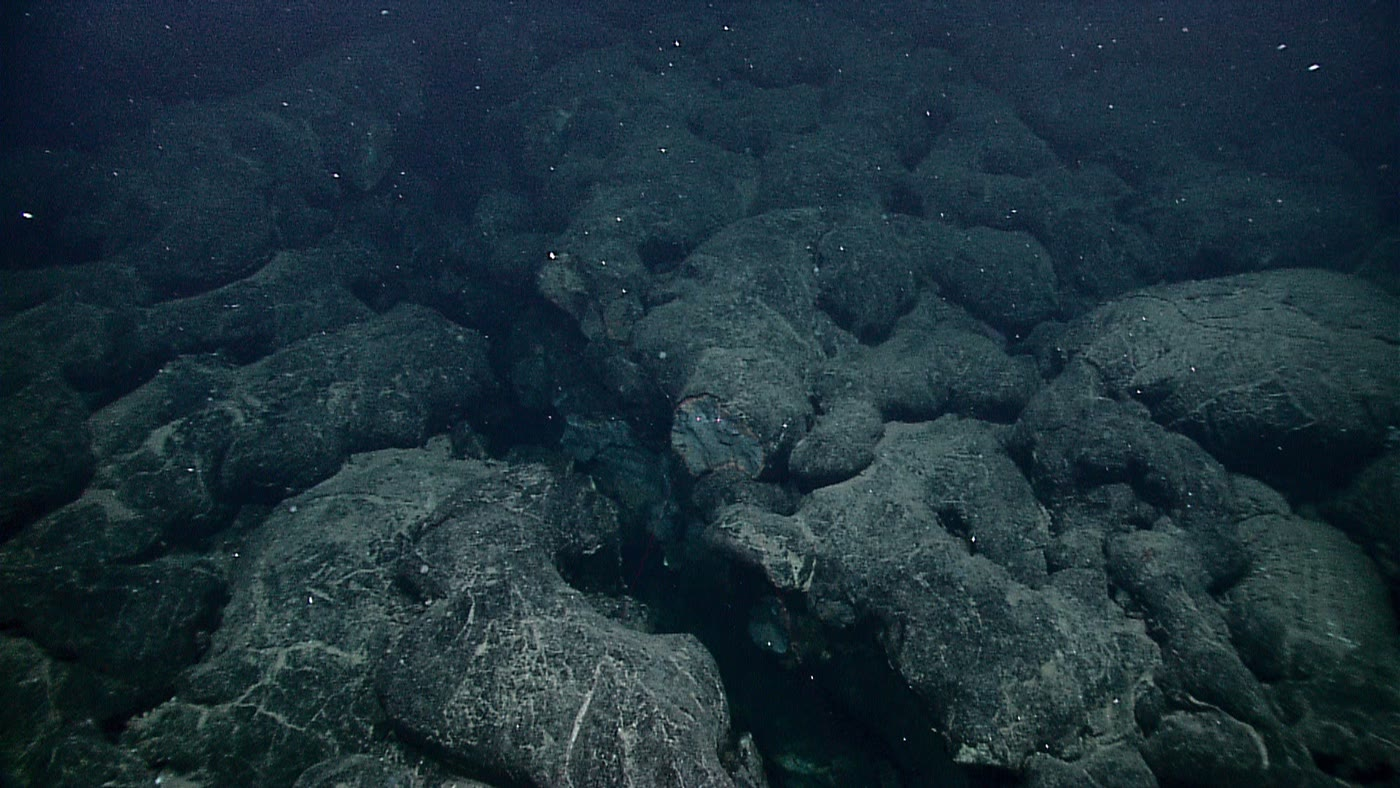
\includegraphics[width=0.6\linewidth]{images/book3/b1-pillow-lava.jpg}

\par\smallskip{\small \omterm{def:b1:rifts-ridges-margins:oceanic-crust}{الحمم الوسادية} على شقّ غالاباغوس، تقطعها شقوق انفتحت بعد أن تصلّبت: أعلى الطبقة~2 من \omterm{def:b1:rifts-ridges-margins:oceanic-crust}{القشرة المحيطية} وهي تتكوّن. وكل وسادة لسانٌ من الحمم جمّدته مياه البحر من الخارج. الصورة: NOAA Okeanos Explorer Program، بعثة شقّ غالاباغوس 2011، CC~BY~2.0 (Wikimedia Commons).}
\label{fig:b1:rifts-ridges-margins:pillows}
\end{omfigure}
% ledger: commons:pillow-expl6453

\begin{proposition}[كل سدّ يشقّ السدّ الذي قبله]\label{prop:b1:rifts-ridges-margins:dykes}
لنفترض أن كل سدّ في \omterm{def:b1:rifts-ridges-margins:oceanic-crust}{مجمع السدود المصفوفة} يتسلّل على امتداد محور الانتشار، حيث \omterm{def:b1:layered-earth:layers}{القشرة} أحرّ ما تكون وأضعف ما تكون، وأن \omterm{def:b1:layered-earth:layers}{القشرة} تتحرّك بعيدًا عن المحور بتماثل. عندئذٍ تُوجد أغلب السدود منشطرةً إلى نصفين، كلٌّ منهما له حافة مبرّدة تجاه جاره الأقدم فقط.
\end{proposition}

\begin{proof}
يتبرّد السدّ عند تماسّه مع الصخر الأبرد على الجانبين، فله حافتان مبرّدتان عند تكوّنه. ويصعد السدّ التالي حيث \omterm{def:b1:layered-earth:layers}{القشرة} أضعف ما تكون، على امتداد المحور، أي عبر وسط السدّ السابق، وهو لا يزال أحرّ الصخور. فيشقّه إلى نصفين، يحملهما الانتشار بعيدًا في الاتجاهين؛ فكل نصف يحتفظ بالحافة المبرّدة على جانبه الخارجي، وله على جانبه الداخلي التماسّ غير المبرّد مع السدّ الجديد. وكل سدّ ما عدا الأخير ينشطر بهذه الطريقة.
\end{proof}

والسدود ذات الحافة المبرّدة على جانب واحد فقط هي فعلًا القاعدة في مجمعات السدود المصفوفة: البصمة \omterm{def:b1:layered-earth:layers}{لقشرة} بُنيت، سدًّا بعد سدّ، بالانتشار.


\section{قانون العمق والعمر}\label{sec:b1:rifts-ridges-margins:depth-age}

قاع المحيط ضحل عند الحيد وعميق بعيدًا عنه. ولأن القاع يتكوّن عند الحيد ويُحمل بعيدًا عنه، فالمسافة عن الحيد هي العمر، وعمق القاع يتعلّق بعمره. وتبرد الصفيحة من أعلى مع تقدّم عمرها (\cref{ch:b1:heat-budget})؛ والصخر البارد أكثف، والعمود الأكثف يطفو أخفض.

\begin{lemma}[تكامل دالة الخطأ]\label{lem:b1:rifts-ridges-margins:erfc}
حيث $\operatorname{erfc} u = 1 - \operatorname{erf} u =
\frac{2}{\sqrt\pi}\int_u^\infty e^{-s^2}\,\mathrm ds$،
\[
  \int_0^\infty \operatorname{erfc} u \,\mathrm du = \frac{1}{\sqrt\pi}.
\]
\end{lemma}

\begin{proof}
مشتقّ $\operatorname{erfc}$ هو $-\frac{2}{\sqrt\pi}e^{-u^2}$. وبالتكامل بالتجزئة على $[0, X]$،
\[
  \int_0^X \operatorname{erfc} u\,\mathrm du
  = \bigl[u \operatorname{erfc} u\bigr]_0^X + \frac{2}{\sqrt\pi}\int_0^X u\,e^{-u^2}\,\mathrm du
  = X\operatorname{erfc} X + \frac{1}{\sqrt\pi}\bigl(1 - e^{-X^2}\bigr).
\]
من أجل $X > 0$ و$s \ge X$، يكون $e^{-s^2} \le (s/X)e^{-s^2}$، إذن
$X\operatorname{erfc} X \le \frac{2}{\sqrt\pi}\int_X^\infty s\,e^{-s^2}\,\mathrm ds
= e^{-X^2}/\sqrt\pi$، وهو يؤول إلى 0. وبجعل $X \to \infty$ نحصل على النتيجة.
\end{proof}

\begin{theorem}[قانون العمق–العمر]\label{thm:b1:rifts-ridges-margins:depth-age}
لنفترض أن
\begin{enumerate}
  \item يغادر \omterm{def:b1:layered-earth:layers}{الوشاح} الحيد عند الحرارة المنتظمة $T_m$، والصفيحة المحيطية ذات العمر $t$ نصف فضاء مبرّد منذ ذلك الحين من سطحه، المحفوظ عند $T_0$، بالانتشارية الحرارية $\kappa$؛
  \item كثافة الصخر المبرّد هي $\rho_m\bigl(1 + \alpha(T_m -
        T)\bigr)$، مع $\rho_m$ كثافة \omterm{def:b1:layered-earth:layers}{الوشاح} عند $T_m$، و$\alpha$ معامل تمدّده الحراري؛
  \item كل عمود في توازن أيزوستاتي فوق عمق تعويض يقع تحت الطبقة المبرّدة، وماء البحر كثافته $\rho_w$.
\end{enumerate}
عندئذٍ يكون عمق قاع البحر ذي العمر $t$
\[
  d(t) = d_r + C\sqrt t, \qquad
  C = \frac{2}{\sqrt\pi}\,\frac{\rho_m\,\alpha\,(T_m - T_0)\sqrt\kappa}{\rho_m - \rho_w},
\]
حيث $d_r$ عمق محور الحيد. وهذا هو \emph{قانون العمق–العمر}\index{قانون العمق–العمر} لقاع المحيط.
\end{theorem}

\begin{proof}
تكون الحرارة في نصف الفضاء المبرّد
\[
  T(z, t) = T_0 + (T_m - T_0)\operatorname{erf}\frac{z}{2\sqrt{\kappa t}},
\]
حيث $z$ العمق تحت قاع البحر؛ وهذا الحل لمعادلة الحرارة يُقبل هنا، كما في \cref{ch:b1:heat-budget}، ويُشتقّ في الكتاب 5.
نقارن العمود عند الحيد، المكوَّن من ماء حتى $d_r$ ومن \omterm{def:b1:layered-earth:layers}{وشاح} عند $T_m$ تحته، بالعمود ذي العمر $t$، المكوَّن من ماء حتى $d$ ومن الصفيحة المبرّدة تحته، وكلاهما حتى \omterm{def:b1:isostasy-gravity:isostasy}{عمق التعويض} $D$. وكتلتاهما لكل وحدة مساحة متساويتان:
\[
  \rho_w d_r + \rho_m (D - d_r) = \rho_w d + \int_0^{D-d}\rho_m\bigl(1 + \alpha(T_m - T)\bigr)\mathrm dz
  = \rho_w d + \rho_m (D - d) + \rho_m\alpha\int_0^{D-d}(T_m - T)\,\mathrm dz.
\]
ومنه
\[
  (\rho_m - \rho_w)(d - d_r) = \rho_m\alpha\int_0^{D-d}(T_m - T)\,\mathrm dz.
\]
بما أن $T_m - T = (T_m - T_0)\operatorname{erfc}\bigl(z/2\sqrt{\kappa t}\bigr)$ مهمل تحت الطبقة المبرّدة، يمكن أخذ التكامل إلى اللانهاية؛ وبوضع $u = z/2\sqrt{\kappa t}$ و\cref{lem:b1:rifts-ridges-margins:erfc}،
\[
  \int_0^\infty (T_m - T)\,\mathrm dz = (T_m - T_0)\,2\sqrt{\kappa t}\int_0^\infty\operatorname{erfc}u\,\mathrm du
  = \frac{2}{\sqrt\pi}(T_m - T_0)\sqrt{\kappa t}.
\]
بالقسمة على $\rho_m - \rho_w$ نحصل على $d - d_r = C\sqrt t$.
\end{proof}

للماء أهميّته: فمع هبوط الصفيحة يملأ الماء الفراغ فوقها، ويدفعها ثقلُه أعمق. ومعامل التمدّد الفعّال $\alpha\rho_m/(\rho_m - \rho_w)$ أكبر من $\alpha$ بالعامل $3300/2300 \approx 1.43$.

مع $\alpha = \qty{3.2e-5}{K^{-1}}$، و$T_m - T_0 = \qty{1350}{K}$، و$\kappa = \qty{e-6}{m^2.s^{-1}}$، و$\rho_m = \qty{3300}{kg.m^{-3}}$ و$\rho_w = \qty{1000}{kg.m^{-3}}$، والزمن معدودًا بالملايين من السنين ($\sqrt{\kappa\times\qty{1}{Myr}} = \qty{5618}{m}$)، تعطي المبرهنة $C = \qty{393}{m.Myr^{-1/2}}$. والثوابت التي ركّبها بارسونز وسكلاتر على أعماق المحيط الهادئ الشمالي والأطلسي الشمالي، بعد إزالة الرواسب، قريبة منها: $d_r \approx \qty{2500}{m}$ و$C \approx \qty{350}{m.Myr^{-1/2}}$، من 0 إلى \qty{70}{Myr}. وقيم $\alpha$ و$T_m$ المستعملة أعلاه هي قيم نموذج صفيحتهما للقاع القديم: \omterm{def:b1:layered-earth:layers}{وشاح} عند \qty{1350}{\degreeCelsius} و$\alpha = \qty{3.2e-5}{\per\degreeCelsius}$، وهي غير مؤكدة بمقدار الخُمس والثلث على التوالي، فإن توافق 393 مع 350 جيّد بقدر ما يُرجى.
% ledger: parsons:plate-model, ps77:depth-age

\begin{example}[قاع محيط عمره 25 و\num{100} مليون سنة]\label{ex:b1:rifts-ridges-margins:depths}
مع $d = 2500 + 350\sqrt t$ (بالأمتار، و$t$ بالملايين من السنين)، يقع القاع البالغ عمره \qty{25}{Myr} عند $2500 + 350\times5 = \qty{4250}{m}$، والقاع البالغ \qty{100}{Myr} عند $2500 + 350\times10 = \qty{6000}{m}$. ويهبط القاع \qty{1750}{m} في أول 25 مليون سنة، ولا يهبط في الخمس والسبعين مليون سنة التالية سوى \qty{1750}{m} أخرى.
\end{example}
% ledger: parsons:plate-model

\begin{omfigure}
\begin{tikzpicture}
\begin{axis}[omrecord, omdepth, width=0.84\linewidth, height=6.6cm,
  xmin=0, xmax=13.6, ymin=2000, ymax=6800,
  xlabel={الجذر التربيعي لعمر القاع، $\sqrt t$ \babelsublr{(\unit{Myr^{1/2}})}},
  ylabel={العمق \babelsublr{(\unit{m})}},
  yticklabel style={/pgf/number format/set thousands separator={}},
  legend style={font=\scriptsize, at={(0.02,0.03)}, anchor=south west, draw=none, fill=white, fill opacity=0.85, text opacity=1},
  legend cell align=left]
% computed in figdata/bachelor-1/depth_age.py; ledger: data:etopo1, data:b2-seafloor-age, parsons:plate-model
\addplot[name path=lo, draw=none, forget plot] table[x expr=sqrt(\thisrow{t}), y=q1] {figdata/out/bachelor-1-depth_age-bins.dat};
\addplot[name path=hi, draw=none, forget plot] table[x expr=sqrt(\thisrow{t}), y=q3] {figdata/out/bachelor-1-depth_age-bins.dat};
\addplot[black!12] fill between[of=lo and hi];
\addlegendentry{النصف الأوسط من الخلايا}
\addplot[only marks, mark=*, mark size=1.1pt, black!70] table[x expr=sqrt(\thisrow{t}), y=median] {figdata/out/bachelor-1-depth_age-bins.dat};
\addlegendentry{العمق الوسيط، فئات عمرية بعرض 2-Myr}
\addplot[very thick, omProp] table[x expr=sqrt(\thisrow{t}), y=halfspace] {figdata/out/bachelor-1-depth_age-models.dat};
\addlegendentry{نصف الفضاء، $2500 + 350\sqrt t$}
\addplot[thick, omDef, densely dashed] table[x expr=sqrt(\thisrow{t}), y=plate] {figdata/out/bachelor-1-depth_age-models.dat};
\addlegendentry{نموذج الصفيحة، $6400 - 3200\,e^{-t/62.8}$}
\draw[black!50, densely dotted] (axis cs:8.944,2000) -- (axis cs:8.944,6800);
\node[font=\scriptsize, anchor=north west, black!70] at (axis cs:8.944,2060) {\qty{80}{Myr}};
\node[font=\scriptsize, anchor=north west, black!70] at (axis cs:4.472,2060) {\qty{20}{Myr}};
\draw[black!50, densely dotted] (axis cs:4.472,2000) -- (axis cs:4.472,6800);
\end{axis}
\end{tikzpicture}

\par\smallskip{\small عمق قاع المحيط بدلالة الجذر التربيعي لعمره. كل نقطة هي العمق الوسيط لخلايا الدرجة الواحدة في محيطات العالم التي يقع قاعها في فئة عمرية بعرض مليونَي سنة (\num{31538} خلية، أعمق من \qty{1000}{m})؛ والنطاق الرمادي يحوي النصف الأوسط منها. وقانون نصف الفضاء خط مستقيم في هذا الرسم. يتبعه القاع الفتيّ عن قرب؛ ويقع القاع الأقدم فوقه، لأن الخلايا تحمل رواسبها وتضم جبالًا بحرية وهضابًا بركانية، ولأن القاع القديم يكفّ عن الهبوط (المتقطّع: نموذج الصفيحة). البيانات: ETOPO1 (NOAA) وأعمار قاع المحيط عند سيتون وآخرين (2020).}
\label{fig:b1:rifts-ridges-margins:depth-age}
\end{omfigure}

يختبر الشكل المبرهنة على المحيط كله. فحتى نحو \qty{20}{Myr} ($\sqrt t \approx 4.5$)، تقع الوسيطات ضمن نحو مائة متر من القانون. ويكون ميل الخط المستقيم المركَّب على الوسيطات الأصغر من \qty{70}{Myr} \qty{250}{m.Myr^{-1/2}} فقط: فالأعماق المقاسة هي أعماق سطح الرواسب، بينما يعطي القانون عمق أعلى \omterm{def:b1:layered-earth:layers}{القشرة}، وغطاء الرواسب يسمك مع العمر. وبين 60 و\qty{80}{Myr}، ينحرف القاع عن قانون الجذر التربيعي حتى بعد إزالة رواسبه: فيصير أضحل من القانون، ويكفّ عن الهبوط. ويصف هذا التسطّح نموذج الصفيحة، وهي صفيحة سمكها \qty{125}{km} قاعدتها مثبّتة عند حرارة \omterm{def:b1:layered-earth:layers}{الوشاح}، فيميل عمقها نحو \qty{6400}{m}، ويميل تدفّقها الحراري إلى قيمة ثابتة، كأن الحرارة تُمدّ إلى قاعدة الصفائح القديمة من \omterm{def:b1:layered-earth:layers}{الوشاح} المتحرّك بالحمل. ويُدرس هذا النموذج في الكتاب 5؛ أما في هذا الكتاب فيُستعمل قانون الجذر التربيعي حتى \qty{80}{Myr}.
% ledger: parsons:plate-model; fit and cell count from depth_age.py (values part)

\begin{method}[تأريخ قاع المحيط من عمقه]\label{met:b1:rifts-ridges-margins:age-from-depth}
لتقدير عمر قاع المحيط حيث تغيب شذوذاته المغناطيسية أو لم تُرسم خرائطها:
\begin{enumerate}
  \item قِس عمق القاع، ومن المقاطع الزلزالية سمك رواسبه؛ وخذ العمق $d$ لأعلى \omterm{def:b1:layered-earth:layers}{القشرة}، مُصحَّحًا بثقل الرواسب؛
  \item اعكس القانون: $t = \bigl((d - d_r)/C\bigr)^2$، مع $d_r$ و$C$ الخاصين بالمحيط المعني؛
  \item تحقّق من أن القاع أصغر من نحو \qty{80}{Myr}، وقدّر عدم اليقين: فخطأ $\delta d$ في العمق يعطي $\delta t = 2t\,\delta d/(d - d_r)$.
\end{enumerate}
\end{method}

بالنسبة إلى قاع عند \qty{4600}{m}، يكون $t = (2100/350)^2 = \qty{36}{Myr}$، وعدم يقين قدره \qty{100}{m} في العمق يعطي $2\times36\times100/2100 \approx
\qty{3.4}{Myr}$ في العمر. وحيث يكون القاع أضحل مما يتنبأ به القانون على مساحة واسعة، أي في انتفاخ، فالسبب ليس العمر بل حرارة من الأسفل (\cref{ch:b1:hotspots}).

ويربط القانون المحيط بمستوى البحر أيضًا. فالحيد الأسرع انتشارًا يحمل القاع الفتيّ الضحل بعيدًا عن محوره؛ فتحتوي أحواض المحيطات ماءً أقل، ويعلو البحر فوق القارات. وعلى مدى عشرات الملايين من السنين، تكون تغيّرات معدّل الانتشار إحدى السببين الرئيسيين لتغيّرات مستوى البحر العالمي، إلى جانب حجم الجليد على اليابسة.

\section{الصدوع التحويلية ومناطق الكسر}

ليست الحيود خطوطًا متصلة: فهي مقطّعة إلى قطع تزيحها صدوع تمتد عموديًا عليها، على امتداد اتجاه الانتشار. وخارج الإزاحات تمتد الصدوع ندوبًا طويلة عبر قاع المحيط.

\begin{definition}[الصدع التحويلي؛ منطقة الكسر]\label{def:b1:rifts-ridges-margins:transform}
\emph{الصدع التحويلي}\index{الصدع التحويلي} صدع انزياحي يكون حدّ صفيحة، وينتهي عند حدود صفائح أخرى؛ والتحويل بين حيد وحيد يصل طرفي قطعتي حيد مزاحتين. و\emph{منطقة الكسر}\index{منطقة الكسر} امتداد الصدع التحويلي خارج طرفي قطع الحيد: واد خطّي أو درجة عبر قاع المحيط تفصل قيعانًا من أعمار مختلفة تنتمي إلى صفيحة واحدة.
\end{definition}

\begin{proposition}[الانزلاق على تحويل بين حيد وحيد]\label{prop:b1:rifts-ridges-margins:transform}
قطعتا حيد تنتشران بتماثل بمعدّل نصفي $u$، عموديًا على نفسيهما، تزيحهما صدع تحويلي طوله $a$. عندئذٍ:
\begin{enumerate}
  \item ينزلق جانبا \omterm{def:b1:rifts-ridges-margins:transform}{الصدع التحويلي} أحدهما عن الآخر بالمعدّل الكامل $2u$، في الاتجاه المعاكس لما توحي به الإزاحة لو كان حيد مستقيم واحد قد قُطع وأُزيح بالصدع؛
  \item على امتداد مناطق الكسر لا يتحرّك الجانبان أحدهما بالنسبة إلى الآخر، ويختلف عمر القاع على الجانبين بمقدار $a/u$؛
  \item طول \omterm{def:b1:rifts-ridges-margins:transform}{الصدع التحويلي} لا يتغيّر مع الزمن.
\end{enumerate}
\end{proposition}

\begin{proof}
خُذ المحور $x$ على امتداد التحويل نحو الشرق، والمحور $y$ نحو الشمال، في إطار الحيد. ليكن القطاع الشمالي على $x = 0$ و$y > 0$، والجنوبي على $x = a$ و$y < 0$ (الإزاحة نحو الشرق عند الاتجاه جنوبًا)؛ والتحويل هو القطعة $0 < x < a$ من $y = 0$. وتقع الصفيحة الغربية $W$ غرب القطعتين وتتحرك بالسرعة $-u$ على امتداد $x$؛ والصفيحة الشرقية $E$ تقع شرقهما وتتحرك بالسرعة $+u$.

(1) مباشرةً شمال التحويل، عند $0 < x < a$، يقع القاع شرق القطعة الشمالية: فهو ينتمي إلى $E$ ويتحرك شرقًا بسرعة $u$. ومباشرةً جنوبه يقع القاع غرب القطعة الجنوبية: فهو ينتمي إلى $W$ ويتحرك غربًا بسرعة $u$. فالجانب الشمالي يتحرك شرقًا بسرعة $2u$ بالنسبة إلى الجانب الجنوبي: ومن أيّ من الجانبين يتحرك الجانب البعيد نحو اليمين، والانزلاق من النوع اليميني. ولو قُطع حيد مستقيم واحد بالصدع، وأصبح جزؤه الجنوبي شرق جزئه الشمالي، لسجّل بدلًا من ذلك إزاحة يسارية.

(2) عند $x > a$، يقع الجانبان شرق قطعتيهما وينتميان إلى $E$: فيتحركان معًا. وعلى المسافة $x$ من القطعة الشمالية، يكون للقاع شمال \omterm{def:b1:rifts-ridges-margins:transform}{منطقة الكسر} العمر $x/u$؛ والقاع جنوبها يبعد $x - a$ عن القطعة الجنوبية، وعمره $(x - a)/u$. والفرق $a/u$. والأمر نفسه عند $x < 0$، حيث ينتمي الجانبان إلى $W$.

(3) تبقى القطعتان عند $x = 0$ و$x = a$ في إطار الحيد، لأن كلًّا منهما ينتشر بتماثل: فيحتفظ التحويل بطوله $a$.
\end{proof}

رأى توزو ويلسون في 1965 أن إزاحات الحيود لا تُقرأ كإزاحة لحيد أقدم مستقيم، وتنبّأ باتجاه الانزلاق الوارد في القضية؛ وأكّدته الآليات البؤرية للزلازل على التحويلات. تقع الزلازل على طول التحويل النشط، بين طرفي الحيد؛ ومناطق الكسر عادةً هادئة. وعبر \omterm{def:b1:rifts-ridges-margins:transform}{منطقة الكسر} يكون لقاعي الجانبين عمران مختلفان، ومن ثمّ، بحسب \omterm{thm:b1:rifts-ridges-margins:depth-age}{قانون العمق–العمر}، عمقان مختلفان: درجة تتلاشى ببطء مع المسافة عن الحيد. وفي شمال الأطلسي قرب \ang{52}~ش، يزيح تحويلا تشارلي–غيبس الحيد الأطلسي الأوسط بنحو \qty{350}{km} في المجموع.
% ledger: wilson:transform, data:pb2002 (offset summed over the transform steps in figdata/bachelor-1/ridge_budget.py)

\begin{omfigure}
\begin{tikzpicture}[x=0.95cm, y=0.95cm, font=\scriptsize]
\fill[omSea!10] (-5,-2.6) rectangle (8,2.6);
% isochrons (10 and 20 Myr), offset across the fracture zones
\foreach \x in {-4,-2,2,4} \draw[black!40] (\x,0) -- (\x,2.5);
\foreach \x in {-1,1,5,7} \draw[black!40] (\x,0) -- (\x,-2.5);
\node[black!55, anchor=south, fill=omSea!10, inner sep=1pt] at (2,2.0) {10};
\node[black!55, anchor=south, fill=omSea!10, inner sep=1pt] at (4,2.0) {20};
\node[black!55, anchor=south, fill=omSea!10, inner sep=1pt] at (-2,2.0) {10};
\node[black!55, anchor=south, fill=omSea!10, inner sep=1pt] at (-4,2.0) {20};
\node[black!55, anchor=north, fill=omSea!10, inner sep=1pt] at (5,-2.0) {10};
\node[black!55, anchor=north, fill=omSea!10, inner sep=1pt] at (7,-2.0) {20};
\node[black!55, anchor=north, fill=omSea!10, inner sep=1pt] at (1,-2.0) {10};
\node[black!55, anchor=north, fill=omSea!10, inner sep=1pt] at (-1,-2.0) {20};
% fracture zones and transform
\draw[black!60, thick, densely dashed] (-5,0) -- (0,0);
\draw[black!60, thick, densely dashed] (3,0) -- (8,0);
\draw[transform, line width=1.4pt] (0,0) -- (3,0);
% ridge segments
\draw[ridge, line width=1.1pt] (0,0) -- (0,2.6);
\draw[ridge, line width=1.1pt] (3,0) -- (3,-2.6);
\pic at (1.5,0) {dextral={90}};
\foreach \x in {0.4,0.75,2.25,2.6} \node[star, star points=5, star point ratio=2.2, fill=orange!90!black, draw=black, line width=0.2pt, inner sep=1.5pt] at (\x,0.0) {};
% plate motions
\draw[-{Stealth[length=4pt]}, very thick, black!70] (-2.8,1.1) -- (-3.9,1.1);
\draw[-{Stealth[length=4pt]}, very thick, black!70] (-0.2,-1.1) -- (-1.3,-1.1);
\draw[-{Stealth[length=4pt]}, very thick, black!70] (5.5,1.1) -- (6.6,1.1);
\draw[-{Stealth[length=4pt]}, very thick, black!70] (5.3,-1.1) -- (6.4,-1.1);
\node[font=\small] at (-3.3,1.55) {الصفيحة $W$};
\node[font=\small] at (6.1,1.55) {الصفيحة $E$};
\node[anchor=west, omRidge] at (0.1,2.25) {حيد};
\node[anchor=east, omRidge] at (2.9,-2.25) {حيد};
\node[anchor=north, align=center, fill=white, fill opacity=0.8, text opacity=1, inner sep=1pt] at (1.5,-0.35) {الصدع التحويلي\\(نشط، زلازل)};
\node[anchor=south, fill=white, fill opacity=0.8, text opacity=1, inner sep=1pt] at (5.5,0.12) {منطقة الكسر (غير نشطة)};
\node[anchor=north, fill=white, fill opacity=0.8, text opacity=1, inner sep=1pt] at (-2.5,-0.12) {منطقة الكسر (غير نشطة)};
\node[anchor=south, black!70, fill=omSea!10, inner sep=1pt] at (6.2,0.55) {أقدم وأعمق};
\node[anchor=north, black!70, fill=omSea!10, inner sep=1pt] at (6.0,-0.45) {أحدث وأضحل};
\end{tikzpicture}

\par\smallskip{\small حيد مزاح بصدع تحويلي، في منظر من أعلى، والشمال إلى الأعلى. تبتعد الصفيحتان عن كل قطعة (الأسهم السوداء)؛ وعلى طول التحويل (الأحمر) تنزلق إحداهما بجانب الأخرى يمينيًا (أنصاف الأسهم)، مع أن إزاحة الحيد تبدو يسارية. والخطوط الرمادية هي خطوط الزمن المتساوي، ومكتوب عليها بملايين السنين: وعبر كل منطقة كسر (متقطعة) يتجاور قاعٌ من أعمار مختلفة، ومن ثمّ أعماق مختلفة، لكن الجانبين يتحركان معًا. النجوم: زلازل، محصورة في التحويل.}
\label{fig:b1:rifts-ridges-margins:transform}
\end{omfigure}

الصدوع التحويلية هي الدليل الثالث على حركات الصفائح في \cref{ch:b1:plate-kinematics}: فالتحويل يمتد على امتداد السرعة النسبية للصفيحتين، فيقع على \omterm{def:b1:spherical-astronomy:spherical-triangle}{دائرة صغرى} حول \omterm{def:b1:plate-kinematics:euler-pole}{قطب أويلر} لهما، وتلتقي الدوائر العظمى المرسومة عموديًا على عدة تحويلات عند القطب. أما مناطق الكسر، المتتبَّعة عبر قاع المحيط، فتسجّل اتجاه الحركة في الماضي، كما تسجّل الشذوذات المغناطيسية معدّلها.

\section{التمارين}

\begin{exercise}[$\star$]\label{exo:b1:rifts-ridges-margins:1}
في 2005 انفتحت قطعة من شقّ عفار طولها \qty{60}{km} بما يصل إلى \qty{8}{m}، وتسلّل \qty{2.5}{km^3} من الصهارة. (أ) لو كان السدّ بسماكة \qty{8}{m} على طول القطعة كلها، فكم كان سيبلغ ارتفاعه المتوسط؟ (ب) بمعدّل الصفيحة \qty{18}{mm.yr^{-1}}، كم سنة من الحركة تمثّل فتحة قدرها \qty{8}{m}؟
% ledger: wright:afar, morvel:ar-nb
\end{exercise}

\begin{exercise}[$\star$]\label{exo:b1:rifts-ridges-margins:2}
نصف غرابن محصور بصدع حدّ إزاحته الرأسية \qty{3.0}{km} ومنحدره \ang{60}، ويقطعه صدع مضادّ أصغر إزاحته الرأسية \qty{0.8}{km} ومنحدره \ang{70}. (أ) احسب \omterm{def:b1:cross-sections:throw}{الإزاحة الأفقية} لكل صدع وامتداد المقطع. (ب) المقطع عرضه الآن \qty{25}{km}: كم كان عرضه قبل الصدوع؟
\end{exercise}

\begin{exercise}[$\star$]\label{exo:b1:rifts-ridges-margins:3}
صنّف الحيود التالية بحدود التعريف، من معدّلات انتشارها الكاملة المحسوبة بمتجهات الصفائح: حيد غاكيل \qty{12}{mm.yr^{-1}}؛ ووسط البحر الأحمر \qty{15}{mm.yr^{-1}}؛ وحيد ريكيانيس \qty{19}{mm.yr^{-1}}؛ وحيد كارلزبرغ الغربي \qty{23}{mm.yr^{-1}}؛ والأطلسي الجنوبي عند \ang{20}~ج \qty{33}{mm.yr^{-1}}؛ وحيد شرق المحيط الهادئ عند \ang{20}~ج \qty{143}{mm.yr^{-1}}. أيّها تتوقّع أن يكون له وادٍ محوري، وأيّها قمّة محورية؟
% ledger: morvel:eu-na, morvel:redsea, morvel:in-sm, morvel:nb-sa, morvel:nz-pa (rates computed with euler_velocities.py)
\end{exercise}

\begin{exercise}[$\star$]\label{exo:b1:rifts-ridges-margins:4}
يتكوّن كل سنة نحو \qty{3.0}{km^2} من قاع بحر جديد، \omterm{def:b1:layered-earth:layers}{بقشرة} سمكها \qty{7.1}{km}. (أ) ما حجم \omterm{def:b1:layered-earth:layers}{القشرة} المتكوّنة كل سنة؟ (ب) بهذا المعدّل، كم يلزم لصنع \qty{3.028e8}{km^2} من قاع المحيط؟ قارن ذلك بعمر أقدم قاع محيطي، نحو \qty{190}{Myr}، وفسّر لماذا لا يلزم أن يتطابق الاثنان.
% ledger: data:pb2002 (ridge_budget.py), white:crust, dd10:split, data:b2-seafloor-age
\end{exercise}

\begin{exercise}[$\star\star$]\label{exo:b1:rifts-ridges-margins:5}
مع $d = 2500 + 350\sqrt t$ (بالأمتار، و$t$ بالملايين من السنين): (أ) احسب عمق القاع البالغ عمره 4 و\num{36} و\num{64} مليون سنة؛ (ب) أوجد عمر القاع الواقع عند \qty{4600}{m} وعند \qty{5300}{m}؛ (ج) بكم ينخفض القاع بين 4 و\qty{36}{Myr}، وبين 36 و\qty{64}{Myr}؟
\end{exercise}

\begin{exercise}[$\star\star$]\label{exo:b1:rifts-ridges-margins:6}
احسب الثابت $C$ \omterm{thm:b1:rifts-ridges-margins:depth-age}{لقانون العمق–العمر} (\cref{thm:b1:rifts-ridges-margins:depth-age}) مع $\alpha =
\qty{3.2e-5}{K^{-1}}$، و$\rho_m = \qty{3300}{kg.m^{-3}}$، و$\rho_w =
\qty{1000}{kg.m^{-3}}$، و$T_m - T_0 = \qty{1350}{K}$ و$\kappa =
\qty{e-6}{m^2.s^{-1}}$، بوحدة \unit{m.Myr^{-1/2}}. أعِد الحساب \omterm{def:b1:layered-earth:layers}{لوشاح} أبرد بمقدار \qty{250}{K}. أيّ ثابت يتبعه قاع محيط أبرد؟
% ledger: parsons:plate-model
\end{exercise}

\begin{exercise}[$\star\star$]\label{exo:b1:rifts-ridges-margins:7}
يعطي نموذج الصفيحة التدفّق الحراري لقاع المحيط بالصيغة $q = 11.3/\sqrt t$، بوحدة \qty{e-6}{cal.cm^{-2}.s^{-1}}، مع $t$ بالملايين من السنين. (أ) حوّل الثابت إلى \unit{mW.m^{-2}.Myr^{1/2}} ($\qty{1}{cal} =
\qty{4.184}{J}$)، وقارنه بالقيمة \qty{490}{mW.m^{-2}.Myr^{1/2}} في \cref{ch:b1:heat-budget}. (ب) احسب $q$ عند 1 و\num{10} و\qty{150}{Myr}. وقد رُكِّب القانون على قاع يصل عمره إلى \qty{120}{Myr}، ويجعل نموذج الصفيحة التدفّق الحراري للقاع الأقدم يستوي عند قيمة ثابتة: فهل القيمة عند \qty{150}{Myr} حينئذٍ أعلى من اللازم أم أدنى؟
% ledger: parsons:plate-model, dd10:young-ocean
\end{exercise}

\begin{exercise}[$\star\star$]\label{exo:b1:rifts-ridges-margins:8}
يمتد حيد في اتجاه شمال–جنوب ويُقطع إلى قطعتين؛ وعند التوجّه جنوبًا على امتداد الحيد، يقفز المحور \qty{40}{km} نحو \emph{الغرب} عند صدع تحويلي. (أ) ما اتجاه الانزلاق على التحويل؟ (ب) ماذا تبيّن إزاحة الحيد على ما يبدو؟ (ج) أين على امتداد خط التحويل تقع الزلازل، ولماذا لا تقع خارجه؟
\end{exercise}

\begin{exercise}[$\star\star$]\label{exo:b1:rifts-ridges-margins:9}
تزيح منطقتا كسر تشارلي–غيبس الحيد الأطلسي الأوسط بمقدار \qty{350}{km} في المجموع؛ والمعدّل الكامل هناك \qty{21.2}{mm.yr^{-1}}. عامِل الإزاحة كتحويل واحد. (أ) ما فرق العمر عبر \omterm{def:b1:rifts-ridges-margins:transform}{منطقة الكسر}؟ (ب) باستعمال $d = 2500 + 350\sqrt t$، احسب فرق العمق عبر \omterm{def:b1:rifts-ridges-margins:transform}{منطقة الكسر} عند نهاية التحويل، ثم على بعد \qty{100}{km} و\qty{1000}{km} بعدها.
% ledger: data:pb2002 (ridge_budget.py), morvel:eu-na (rate at 52.5 N 31.5 W from euler_velocities.py)
\end{exercise}

\begin{exercise}[$\star\star\star$]\label{exo:b1:rifts-ridges-margins:10}
يُنشأ حوض محيطي بمعدّل ثابت، ويحوي قاعًا من كل عمر من 0 إلى $A$ على مساحات متساوية. (أ) أثبت أن عمقه المتوسط هو $d_r +
\frac23C\sqrt A$. (ب) مع $d_r = \qty{2500}{m}$ و$C = \qty{350}{m.Myr^{-1/2}}$، قارن $A = \qty{180}{Myr}$ و$A = \qty{120}{Myr}$. (ج) لو تسارع انتشار الحوض بحيث يصبح أقدم قاعه \qty{120}{Myr} بدلًا من \qty{180}{Myr}، فبكم يرتفع مستوى البحر، مع إهمال غمر القارات لكن مع احتساب حمل الماء الإضافي على القاع الذي يهبط بمقدار $\rho_w/(\rho_m - \rho_w)$ من الارتفاع ($\rho_m = 3300$، $\rho_w = \qty{1000}{kg.m^{-3}}$)؟
\end{exercise}

\begin{exercise}[$\star\star\star$]\label{exo:b1:rifts-ridges-margins:11}
في إطار \cref{prop:b1:rifts-ridges-margins:transform}، فرق العمق عبر منطقة كسر على المسافة $x > a$ من قطعة الحيد الأبعد هو $\Delta d = C\bigl(\sqrt{x/u} - \sqrt{(x - a)/u}\bigr)$. (أ) أثبت أنه من أجل $x \gg a$، يكون $\Delta d \approx Ca/(2\sqrt{ux})$. (ب) مع $C = \qty{350}{m.Myr^{-1/2}}$، و$a = \qty{350}{km}$، و$u = \qty{10.6}{km.Myr^{-1}}$، قارن الفرقين الدقيق والتقريبي عند $x = 450$ و\num{1350} و\qty{3350}{km}. متى يكون التقريب جيدًا بنسبة \qty{10}{\percent}؟
\end{exercise}

\begin{exercise}[$\star\star\star$]\label{exo:b1:rifts-ridges-margins:12}
قارِن قانون نصف الفضاء $d_1(t) = 2500 + 350\sqrt t$ بقانون الصفيحة $d_2(t) = 6400 - 3200\,e^{-t/62.8}$. (أ) احسب $d_2 - d_1$ عند 10 و\num{20} و\num{30} و\qty{40}{Myr}. (ب) بيّن أن القانونين متساويان عند عمر واحد بين 20 و\qty{30}{Myr}، وأوجِده إلى \qty{0.1}{Myr} بالتنصيف المتكرر. (ج) قارن ميليهما هناك. لماذا يمكن وصل القانونين عند ذلك العمر دون انكسار مرئي؟
% ledger: parsons:plate-model
\end{exercise}

\section{مسألة: ولادة محيط}

\begin{problem}[{مسألة نهاية الأسبوع: قارة تتمدّد بصدوعها، ومحيط فتيّ يُقاس بخطوطه، وعمق قاعه مع تقدّم عمره}]
\label{pb:b1:rifts-ridges-margins:1}
% values: calc/ch13.py (Part I rift section and Part II profile invented for the
% problem; real Euler vector, chron ages and depth--age constants)
% ledger: morvel:sm-an, morvel:nb-an, morvel:ar-nb, morvel:redsea, morvel:outward, iodp:gpts2004, heine:sam-saf, parsons:plate-model, wright:afar
خذ $R = \qty{6371}{km}$. يولد محيط في ثلاث مراحل، يُرى كل منها اليوم في مكان مختلف: شقّ قاري، ومحيط فتيّ، ومحيط قديم.

\medskip
\noindent\textbf{الجزء الأول --- شقّ تمدّده صدوعه.} يقطع مقطعٌ عبر شقّ يمتد باتجاه \ang{020} ستةَ صدوع عادية، قيست إزاحاتها الرأسية وانحداراتها على المقاطع الزلزالية:
\begin{center}
\small
\begin{tabular}{lcccccc}
\hline
الصدع & F1 & F2 & F3 & F4 & F5 & F6\\
\omterm{def:b1:cross-sections:throw}{الإزاحة الرأسية} (\unit{m}) & \mbox{\textdir TLT 600} & \mbox{\textdir TLT 1100} & \mbox{\textdir TLT 2400} & \mbox{\textdir TLT 350} & \mbox{\textdir TLT 800} & \mbox{\textdir TLT 1500}\\
\omterm{def:b1:geological-maps:attitude}{الانحدار} & \mbox{\textdir TLT \ang{60}} & \mbox{\textdir TLT \ang{55}} & \mbox{\textdir TLT \ang{50}} & \mbox{\textdir TLT \ang{65}} & \mbox{\textdir TLT \ang{60}} & \mbox{\textdir TLT \ang{52}}\\
\hline
\end{tabular}
\end{center}
تقطع الصدوع حممًا عمرها \qty{3.2}{Ma}، والشقّ عرضه الآن \qty{60}{km}.
\begin{enumerate}
  \item احسب \omterm{def:b1:cross-sections:throw}{الإزاحة الأفقية} لكل صدع. أيّها صدع الحدّ؟
  \item احسب امتداد المقطع، وعرض الشقّ قبل الصدوع.
  \item تتباعد الصفيحتان بمعدّل \qty{6.0}{mm.yr^{-1}} نحو \ang{105}. احسب مركبة هذه الحركة العمودية على الشقّ.
  \item كم يلزم للصفيحتين لتُنتجا امتداد السؤال 2؟
  \item بكم تباعدت الصفيحتان منذ ثوران الحمم؟ وما الكسر الذي تحمله الصدوع منه؟
  \item اقترح أين ذهب باقي \omterm{def:b1:geological-maps:attitude}{الامتداد}. ولو استوعبته سدود مثل سدّ عفار عام 2005، عرض كل منها \qty{8}{m}، فكم سدًّا يلزم، وكم مرة؟
\end{enumerate}

\medskip
\noindent\textbf{الجزء الثاني --- محيط فتيّ يُقاس بخطوطه.} قطاع مغناطيسي عبر محور وسط البحر الأحمر، عند \ang{18.0}~ش و\ang{40.0}~ق، يمتد على امتداد اتجاه الانتشار. الحافة الحديثة للحقبة C2An (\qty{2.581}{Ma}) تقع على \qty{21.0}{km} شمال شرق المحور و\qty{20.2}{km} جنوب غرب، والحافة القديمة للحقبة C3n (\qty{5.235}{Ma}) تقع على \qty{41.0}{km} و\qty{40.2}{km}. وحافات الشذوذات مزاحة إلى الخارج عن المحور بمقدار \qty{2.2}{km} في المجموع، في المتوسط، على الجانبين معًا.
\begin{enumerate}[resume]
  \item احسب \omterm{def:b1:plate-kinematics:spreading-rate}{معدّل الانتشار الكامل} من كل حقبة، دون تصحيح.
  \item صحّح كل معدّل للإزاحة إلى الخارج. هل يتفق المعدّلان؟
  \item أثبت أن المعدّل المحسوب من المسافة بين الحقبتين على كل جانب لا يحتاج إلى تصحيح، واحسبه.
  \item احسب المعدّلين النصفيين على كل جانب من المسافات بين الحقبتين. هل الانتشار متماثل؟
  \item \omterm{def:b1:plate-kinematics:euler-pole}{قطب أويلر} للصفيحة العربية بالنسبة إلى النوبية عند \ang{30.9}~ش و\ang{23.6}~ق، بمعدّل \qty{0.403}{\degree\per\Myr}. احسب البعد الزاوي من القطب إلى القطاع، \omterm{def:b1:plate-kinematics:spreading-rate}{ومعدّل الانتشار الكامل} الذي تتنبأ به متجهة الصفيحة هناك.
  \item في شمال البحر الأحمر، عند \ang{26.0}~ش و\ang{35.0}~ق، احسب البعد الزاوي من القطب والمعدّل المتنبأ به.
  \item قارن هذه المعدّلات بالمقاسة، 15 و\qty{9}{mm.yr^{-1}}. لماذا ينفتح البحر الأحمر أسرع في الجنوب؟
\end{enumerate}

\medskip
\noindent\textbf{الجزء الثالث --- نحو أطلسي.}
\begin{enumerate}[resume]
  \item ما عرض قاع المحيط المتكوّن في وسط البحر الأحمر منذ الحافة القديمة للحقبة C3n، بمعدّل السؤال 9؟
  \item فتح الأطلسي الجنوبي بنحو \qty{5000}{km} عند ريسيفي خلال \qty{120.6}{Myr} (\cref{ch:b1:plate-kinematics}). احسب معدّل انفتاحه المتوسط.
  \item بالمعدّل الحالي لوسط البحر الأحمر، كم يستغرق انفتاح قدره \qty{5000}{km}؟ وبمعدّل شماله؟
  \item ينفتح البحر الأحمر حول قطب قريب منه. ماذا يعني ذلك لشكله وهو يتّسع، ولمدة الجزء الشمالي اللازمة ليبلغ العرض الذي يبلغه الجزء الأوسط الآن؟
  \item أيّ نوع من الحيود محورُ البحر الأحمر، وأيّ شكل للمحور تتوقّع؟
\end{enumerate}

\medskip
\noindent\textbf{الجزء الرابع --- القاع يهبط.} استعمل $d = 2500 + 350\sqrt t$ (بالأمتار، و$t$ بالملايين من السنين)، وللمقارنة قانون الصفيحة $6400 - 3200\,e^{-t/62.8}$.
\begin{enumerate}[resume]
  \item احسب عمق القاع الجديد عند الأعمار 1 و\num{10} و\qty{40}{Myr}.
  \item في أيّ عمر يبلغ القاع \qty{4000}{m}؟
  \item القاع المجاور لكل هامش سلبي عمره عمر المحيط. بكم ينخفض في أول \qty{10}{Myr} بعد الانفصال، وبين 70 و\qty{80}{Myr}؟
  \item بأي معدّل، بالأمتار لكل مليون سنة، ينخفض ذلك القاع عندما يبلغ عمر المحيط \qty{80}{Myr}؟
  \item ما التدفّق الحراري الذي يفقده قاع السؤال 22 عندئذٍ، مع $q = 490/\sqrt t$ بوحدة \unit{mW.m^{-2}}؟
  \item احسب عمق قاع عمره \qty{80}{Myr} بكل من القانونين، وفرقهما. لماذا يجوز مقارنة القانونين عند هذا العمر؟
  \item بأقرب عُشر من الكيلومتر، ما عمق قاع البحر الجديد عند عمر 80 مليون سنة وفق قانون الجذر التربيعي؟
\end{enumerate}
\end{problem}
